\documentclass[10pt]{article}
\usepackage[margin=0.82in]{geometry}
\usepackage[T1]{fontenc}
\usepackage{amsmath,amssymb,booktabs,longtable,hyperref,tikz}
\usetikzlibrary{arrows.meta,positioning}
\hypersetup{colorlinks=true,urlcolor=blue}
\title{\textbf{Fractal Holonet: 40 Programmable Four-Port Buses}\\
An Exact W33 Incidence and Quantum-Optical Switching Blueprint}
\author{W33-Theory engineering programme}
\date{23 October 2026 --- executable graph and target-unitary release}
\begin{document}\maketitle
\begin{abstract}
The previously established W33 line decomposition supplies 40 four-point
buses covering 240 pairwise edges. This addendum lowers that finite
geometry into a concrete architecture of 40 programmable four-port optical
exchange \emph{targets} per 40-child parent. Three exact $4\times4$
permutation matrices per bus schedule every W33 neighbor-pair once in
three slots; the same model specifies recursive bus-to-child portal
mapping and provides a complete level-two graph with 1,600 vertices and
exact diameter six. The buses remain mathematical optical circuits;
no PDK, waveguide layout, electrodes, fabrication, time-of-flight data,
or quantum-hardware measurements are claimed.
\end{abstract}
\tableofcontents
\section{What is prior art; what is newly implemented here}
The 40-point collinearity graph and its 40 isotropic lines belong to
$W(3,3)$ itself. \texttt{analysis/w33\_scheduler\_os.py} had
\emph{already} computed the 40 four-way line-bus map and the
12-perfect-matching single-port schedule. We do not present
those combinatorial facts as new discoveries.
The additional engineering construction is (1) explicit
three-state four-port \emph{quantum-optical permutation matrices},
(2) a four-independent-bus-ports-per-child concurrency
contract, and (3) a fully executable recursive leaf graph
using separate, indexed ingress and egress portal addresses.

\section{Geometry and physical bus interface}
The symplectic pairing is
\[
\langle u,v\rangle
=u_0v_1-u_1v_0+u_2v_3-u_3v_2\pmod3.
\]
Distinct points are collinear iff this pairing vanishes.
There are 40 points, 240 edges, and 40 four-point lines.
Every point belongs to exactly four lines, and every edge
belongs to exactly one line. Therefore one 40-child parent has
exactly 40 \emph{four-terminal} buses and 160 child-to-bus
incidences. Each child requires four independent bus-access ports
rather than twelve pairwise-neighbor terminations.

\begin{center}
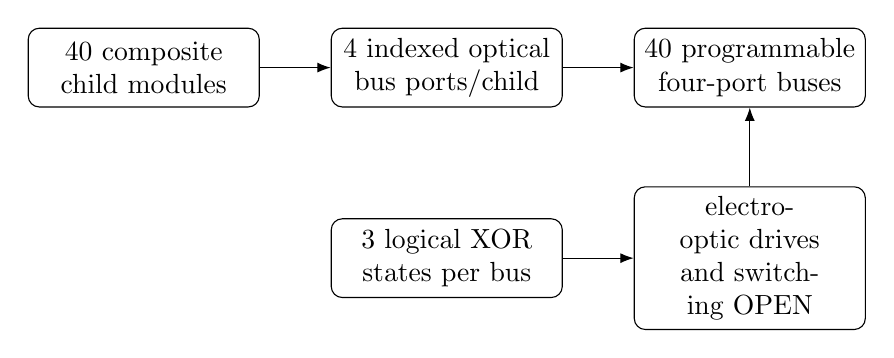
\begin{tikzpicture}[>=Latex,blk/.style={draw,rounded corners,align=center,text width=27mm,minimum height=10mm},node distance=9mm]
\node[blk](host){40 composite\\child modules};
\node[blk,right=of host](ports){4 indexed optical\\bus ports/child};
\node[blk,right=of ports](bus){40 programmable\\four-port buses};
\node[blk,below=10mm of bus](drive){electro-optic drives\\and switching OPEN};
\node[blk,left=of drive](state){3 logical XOR\\states per bus};
\draw[->](host)--(ports);\draw[->](ports)--(bus);
\draw[->](state)--(drive);\draw[->](drive)--(bus);
\end{tikzpicture}
\end{center}
This is \emph{not} a passive four-way broadcast medium:
two disjoint pairs must be switched independently on the same
four-port bus in one timeslot. Therefore all optical ports,
switch couplers, path crossings, phase actuators and electrical
control signals still require explicit physical engineering.

\section{The Klein-four permutation program}
Order a bus's four ports by two-bit labels $0,1,2,3$.
For each two-bit mask $m$, define the real permutation matrix
\[
(P_m)_{j,k}=
\begin{cases}
1&j=k\oplus m,\\
0&\text{otherwise}.
\end{cases}
\]
These matrices obey
\[
P_m^\dagger P_m=I_4,\quad
P_m P_n=P_{m\oplus n},\quad
P_m^2=I_4,\quad \det(P_m)=+1.
\]
The three nonidentity masks are exactly the three perfect
matchings of a complete four-node line:
\[
\begin{array}{rcl}
m=01 &: &(0\leftrightarrow1),\ (2\leftrightarrow3),\\
m=10 &: &(0\leftrightarrow2),\ (1\leftrightarrow3),\\
m=11 &: &(0\leftrightarrow3),\ (1\leftrightarrow2).
\end{array}
\]
Thus the switch states constitute the Klein four-group
$C_2\times C_2$. This is a \emph{particularly simple}
subgroup of $SO(4)$, not a demand for fully programmable
$U(4)$ on every bus.
A general $4\times4$ unitary interferometer would need six
two-mode mixing cells in standard Reck/Clements-style synthesis;
40 such fully configurable meshes suggest 240 two-mode cells
per parent as a \emph{generic upper architecture model}.
A fixed-function device implementing only these three
permutations could require materially fewer resources.
Without a selected optical PDK and actual coupler/drive
topology, neither number is a fabrication result.

\section{Exact three-slot parent network schedule}
At each slot every bus performs one of the three pairings.
A four-point line contributes two disjoint neighbor pairs,
so 40 buses concurrently offer $40\cdot2=80$ pair
communications. Since each point lies on four lines, each
child uses exactly four distinct bus ports per slot.
Over three slots, each of the 240 W33 edges is covered
once. With at most four simultaneous neighbor connections
per child, the lower bound $\lceil12/4\rceil=3$ slots is
attained in this \emph{specified logical service model}.

\section{Recursive lowering and shortest paths}
Each child belongs to four distinct parent lines.
Map those four parent-bus identifiers, in a declared
sorted order, to four gateway addresses on one selected
child line $L=(0,31,32,33)$. This is a \emph{chosen
gauge/address convention}, not a symmetry-forced identity.
The source and destination gateway digit for an inter-child
edge can differ, so one parent-bus crossing can change
two address digits. Counting it as a single physical
connection is valid only because the four-port bus
is explicitly part of the topology.
The executable recursive graph connects these physical
portal addresses and retains ordinary W33 adjacency in
each lowest-level child.
Exhaustive breadth-first search over all 1,600 depth-two
leaves gives exact diameter $6$ and eccentricity
multiplicities $5^{160}+6^{1440}$.
This compares with diameter $4$ for the Cartesian
model, $5$ for the fully replicated gateway model,
and $7$ for the one-edge-per-neighbor sparse
matched-gateway design; these are four distinct networks.

\section{Physical sign-off gates}
\begin{longtable}{p{0.29\linewidth}p{0.56\linewidth}}
\toprule
Subsystem & Needed before an optical hardware claim\\\midrule
Optical crossbar & A measured or process-modelled
4-by-4 scattering matrix for all 3 permutation states\\
PIC layout & Port-orientation-correct PDK waveguides,
couplers, phase shifters, bends/crossings, DRC and optical LVS\\
Drive electronics & The physical mapping from the logical
two-bit slot selector to all real electrodes, settling time
and clock synchronization\\
Loss and leakage & Frequency/polarization response,
per-state insertion loss, phase drift, excess extinction
and two-photon characterization where appropriate\\
Packet scheduling & Switch guard times, buffers, busy
ports, fairness, congestion and fault recovery\\
Hierarchy & Optical packaging across 40-child modules,
path-loss scaling and admissible quantum-source budgets\\
\bottomrule
\end{longtable}
The earlier two-MZI 1-to-3 gateway selector surrogate is a
\emph{different physical design alternative}, not the
four-port bus implementation. Its illustrative phase/loss
parameters cannot be transferred to a four-port switch
without an explicit component derivation.

\section{Executable files and verification}
The principal implementation is
\texttt{analysis/w33\_fractal\_linebus\_switch\_matrix\_20261023.py}.
Its frozen certificate and 40-bus-by-three-slot matrix schedule
appear in
\texttt{data/w33\_fractal\_linebus\_switch\_matrix\_20261023.json}.
Regression tests are in
\texttt{tests/test\_w33\_fractal\_linebus\_switch\_matrix\_20261023.py}.
The source validates all 40 incidence lines, 240 unique edges,
all three $4\times4$ exact unitary permutation programs,
all 160 bus endpoint incidences, recursive route legality,
and the 1,600-source level-two BFS diameter.
This is an executable \emph{design} and mathematical witness,
not a built, calibrated, or universal photonic computer.
\end{document}
